\documentclass[tikz,border=10pt]{standalone}
\begin{document}
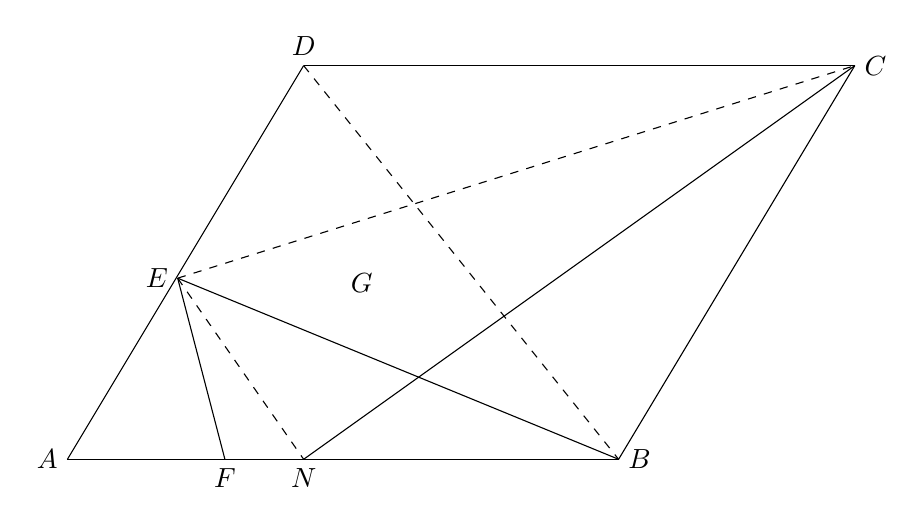
\begin{tikzpicture}[scale=1]

% Coordinates
\coordinate (A) at (0,0);
\coordinate (B) at (7,0);
\coordinate (C) at (10,5);
\coordinate (D) at (3,5);
\coordinate (E) at (1.4,2.3);
\coordinate (F) at (2.0,0);
\coordinate (N) at (3.0,0);
\coordinate (G) at (4.0,2.0);

% Outer shape
\draw (A) -- (B);
\draw (B) -- (C);
\draw (D) -- (C);
\draw (A) -- (D);

% Inner solid segments
\draw (E) -- (F);
\draw (E) -- (B);
\draw (N) -- (C);

% Dashed segments
\draw[dashed] (E) -- (C);
\draw[dashed] (D) -- (B);
\draw[dashed] (E) -- (N);

% Labels
\node[left] at (A) {$A$};
\node[right] at (B) {$B$};
\node[right] at (C) {$C$};
\node[above] at (D) {$D$};
\node[left] at (E) {$E$};
\node[below] at (F) {$F$};
\node[below] at (N) {$N$};
\node[above left] at (G) {$G$};

\end{tikzpicture}
\end{document}
